\section{Desarrollo y modificaciones de la arquitectura}

En este capítulo, se introducen los cambios y desarrollos principales que se han llevado a cabo durante el trabajo.

\subsection{Cloud} 

Con el objetivo de reducir el tiempo necesario para entrenar los distintos modelos que se plantean en este trabajo, se ha recurrido al servicio de infraestructura (IaaS - \textit{Infraestructure as a Service}) que ofrece la empresa Google: Google Cloud. Los servicios en la nube (\textit{cloud}), permiten disponer de recursos informáticos de manera flexible, pagando únicamente por aquellos que estén activos. Los proveedores de IaaS, se encargan del mantenimiento y gestión de la infraestructura (redes, almacenamiento, servidores, virtualización), mientras que el usuario se encarga de la gestión del sistema operativo y todo lo que hay por encima. 

Dentro de Google Cloud, se han empleado los servicios \textbfit{Compute Engine}, para disponer de máquinas virtuales y \textbfit{Cloud Storage}, para crear recursos de almacenamiento (\textit{buckets}).

El flujo de trabajo que se ha seguido ha sido el siguiente (\ref{fig:cloud-diagram}):

\begin{enumerate}
\item Primero, se ha creado un \textit{bucket} en el que se han dejado disponibles el conjunto de datos empleado durante el entrenamiento, el código necesario para ejecutar el entrenamiento, y una serie de scripts para facilitar la configuración del equipo. Al disponer de estos archivos en la nube, se desacoplan totalmente la configuración de las máquinas virtuales y el ordenador local en el que se lleva a cabo el desarrollo (Equipo 1 en Tabla \ref{tab:computer-specs}).
\item A continuación, se configura una máquina virtual con el \textit{hardware} elegido\footnote{Para elegir el \textit{hardware} de las máquinas virtuales, se ha elegido la GPU que mayor relación TFLOPS/euro ofrecía para minimizar el coste de los equipos. El resto de características se han elegido de forma que la limitación del equipo sea el procesamiento en GPU.} (Equipo 2 en Tabla \ref{tab:computer-specs}). Una vez conectados a esta máquina virtual a través de SSH, se descarga del \textit{bucket} creado el script de configuración (disponible en el Anexo TODO) y se ejecuta. Este script, se encarga de: descargar el resto de archivos disponibles en el \textit{bucket}, instalar los drivers de NVIDIA necesarios para poder usar la GPU de la instancia, instalar Docker y el NVIDIA Container Toolkit, instalar Weights and Biases, y construir la imagen de Docker especificada en el Dockerfile descargado.
\item Una vez configurada la instancia con todos los archivos necesarios en su disco SSD, se crea una imagen de dicha instancia en Google Cloud de forma que sea fácilmente replicable. Posteriormente, se configura desde la consola de Google Cloud el inicio de estas instancias de forma que cada vez que se encienda una (nueva o ya existente), se cree dentro del equipo un contenedor de Docker a partir de la imagen ya construida, y se ejecute en este contenedor el cliente de Weight and Biases para entrenar modelos automáticamente. De esta forma, para añadir una nueva máquina al proceso de entrenamiento de experimentos, solamente hay que crear un nuevo equipo a partir de la imagen preconfigurada.
\item Por último, una vez finalizados los experimentos, se copia a través de SSH los parámetros de los modelos entrenados, que se han guardado en cada una de las máquinas virtuales empleadas.
\end{enumerate}

\begin{figure}[H]
\centering
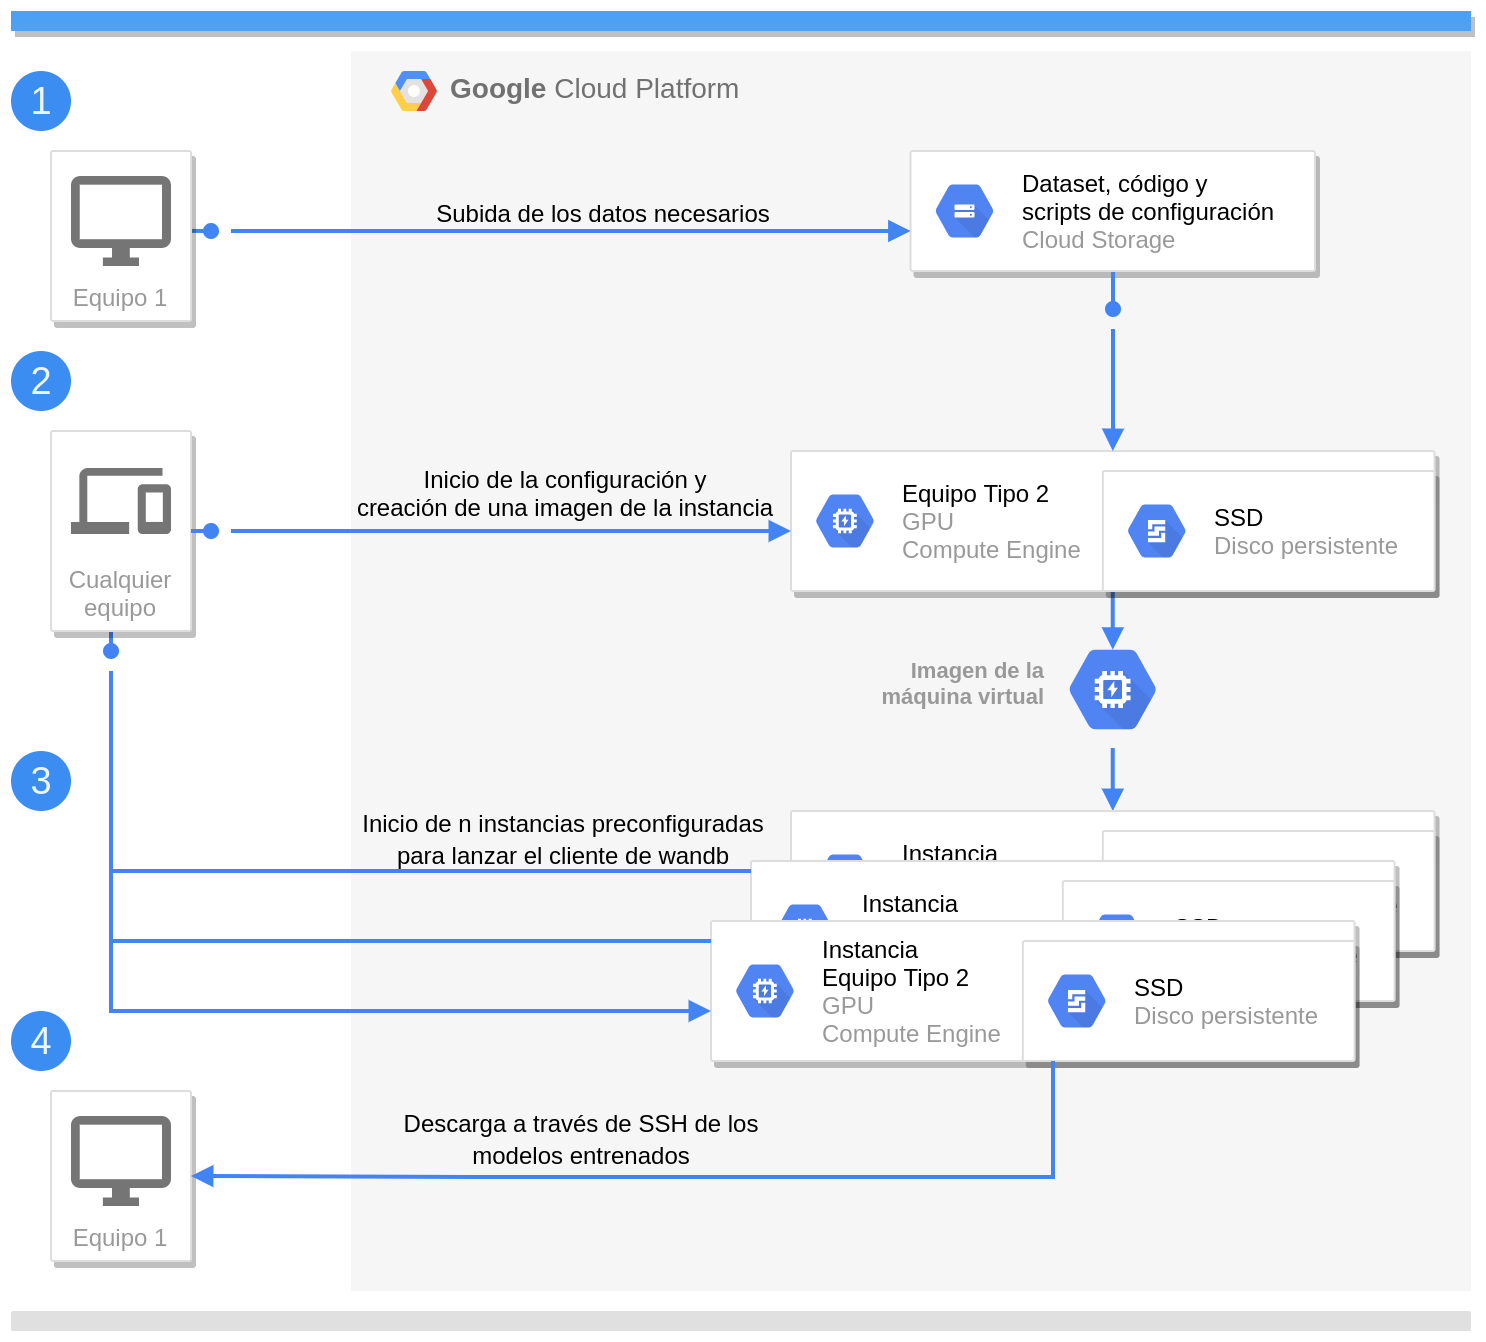
\includegraphics[width=\textwidth]{imagenes/cloud-diagram.png}
\caption{Esquema de la configuración llevada a cabo en la nube.}
\label{fig:cloud-diagram}
\end{figure}

\subsection{Warmstart}
Para acelerar lo máximo posible la convergencia del modelo durante el entrenamiento, se aprovechan en la medida de lo posible parámetros con sesgos inductivos ya aprendidos, es decir, parámetros de modelos ya entrenados. Más concretamente, los parámetros de los modelos a entrenar se inicializan con los valores de los parámetros del modelo DPT-Hybrid entrenado en MIX6, publicados en el artículo original de \textit{Dense Prediction Transformers} \cite{visiontransformersDPT}. 

Además, ya que en este trabajo se estudian diferentes modificaciones de dicho modelo, se emplea el método \texttt{load\_state\_dict()} de la clase \texttt{torch.nn.Module} con el parámetro \texttt{strict=False} para cargar los parámetros, evitando así que la carga falle si no coinciden una a una las capas en el modelo y las definidas en el archivo que se trata de cargar. En cuanto a las capas/conjuntos de capas que se han modificado y/o añadido, al no disponer del conjunto de datos MIX6 para preentrenarlas, se han inicializado con sus parámetros correspondientes tras ser entrenadas en ImageNet21K.

\todo[inline]{Comprobar esto entrenando el modelo de ResNet con los pesos de imagenet.}
Esta forma de proceder, sin embargo, origina un problema que se comentará más adelante en detalle, y es que como era de esperar, los modelos con menor porcentaje de su arquitectura modificada parten de una situación inicial ventajosa para la tarea de estimación de profundidad monocular (al estar preentrenados en MIX6).

\subsection{Entrenamiento}
Pese a que los autores del artículo de DPT \cite{visiontransformersDPT} han publicado el código del modelo y sus pesos preentrenados en MIX6 y KITTI, a día de hoy no han hecho público los \textit{scripts} de entrenamiento empleados. Por esto, ha sido necesario escribir el proceso de entrenamiento así como el \texttt{Dataset} de PyTorch con el que leer los datos de KITTI.

Para el \texttt{Dataset}, se crea una clase \texttt{KITTIDataset}\footnote{URL al repo?} que hereda de la clase abstracta base para conjuntos de datos que ofrece PyTorch, \texttt{torch.utils.data.Dataset}, y sobreescribe los métodos \texttt{\_\_len\_\_()} y \texttt{\_\_getitem\_\_()} de forma que estos se adapten a la estructura de directorios y nombres de las imágenes de sus anotaciones. Al sobreescribir estos métodos, es posible crear un \texttt{torch.utils.data.Dataloader} de forma directa, pasando las imágenes y las etiquetas a los modelos aprovechando las herramientas de PyTorch. En el método \texttt{\_\_getitem\_\_()}, además, se aplican las transformaciones necesarias a los datos, así como el \textit{Data Augmentation}.

Por \textit{Data Augmentation} se entiende el conjunto de operaciones y transformaciones que se pueden aplicar a los datos para modificar su apariencia. Esto, normalmente favorece el aprendizaje y la capacidad de generalización de la red (tiene efecto regularizador y evita el sobreajuste al aumentar el número de ejemplos y la variedad entre ellos). En el entrenamiento llevado a cabo, siguiendo una vez más la metodología de DPT, se ha incluido un \textbf{reflejado horizontal aleatorio}, es decir, cada una de las imágenes (junto con las anotaciones) tiene un $50\%$ de posibilidades de ser reflejada horizontalmente antes de atravesar la red como ejemplo de entrenamiento.

En cuanto al \textit{script} de entrenamiento\footnote{URL de train.py y train\_ utils.py?}, se tienen en cuenta una serie de factores para acelerar el proceso lo máximo posible:
\begin{itemize}

\item \textbf{Número de trabajadores en el \texttt{Dataloader}}: Con el objetivo de asegurar que la limitación en la velocidad de entrenamiento sea el procesamiento en la GPU, se cambia el valor del parámetro \texttt{num\_workers} del constructor del \texttt{Dataloader} de entrenamiento a 8. Este parámetro, controla el número de procesos que se lanzan en paralelo para leer los datos del disco y preprocesarlos.

\item \textbf{\texttt{pin\_memory}}: También en el constructor del \texttt{Dataloader}, es posible activar \texttt{pin\_memory}, parámetro desactivado por defecto. Este parámetro, acelera la transferencia a la memoria de la GPU de los datos cargados en memoria (RAM) por la CPU \cite{harris2012}. De forma resumida, lo que habilita este parámetro es que la carga de datos se haga en memoria no paginable (\textit{pinned}) a la que la GPU accede directamente, evitando así cargar los datos en una zona de memoria paginable y transferir estos a una \textit{pinned memory} temporal cada vez que la GPU quiere leerlos para transferirlos a su propia memoria.

\item \textbf{\texttt{torch.backends.cudnn.enabled y \texttt{torch.backends.cudnn.benchmark}}}: Estas dos opciones, se activan para asegurar, respectivamente, que se use CuDNN en la ejecución del modelo y que se ejecuten al comienzo del \textit{script} distintas implementaciones de algoritmos de convolución para emplear el más rápido en el sistema actual.

\item \textbf{\textit{Mixed precision}}: Ya mencionado en el apartado TODO, pese a que finalmente se ha descartado su uso en el entrenamiento debido a la inestabilidad numérica que introducía y los fallos que ocasionaba, el \textit{script} de entrenamiento incluye la opción de activar el uso de precisión mixta con el escalado pertinente.
\end{itemize}

\todo[inline]{Medir y hacer una gráfica de la influencia de cada uno de estos en un trozo de epoch}

Para ajustar los parámetros de los modelos, se ha empleando como optimizador \texttt{AdamW} con una tasa de aprendizaje $lr = 1e-5$ y parámetros: $\beta_1 = 0.9$, $\beta_2 = 0.999$, $\epsilon = 1e-8$ y $\textit{weight decay} = 0.01$. El número de épocas se ha fijado en $20$ tras analizar el comportamiento de la pérdida en distintas ejecuciones. En cuanto al tamaño de lote usado, se ha utilizado solamente una imagen para cada actualización de parámetros. Esta elección viene motivada por dos razones, la primera, la falta de recursos computaciones para entrenar algunas de las variaciones de los modelos con lotes de más imágenes, y la segunda y más importante, que tras implementar en el \textit{script} de entrenamiento la posibilidad de acumular gradientes\footnote{La acumulación de gradientes (\textit{gradient accumulation}) es una técnica que promedia las pérdidas en distintos lotes para, aún sin poder aprovechar la mejora de rendimiento de un tamaño de lote mayor, conseguir que la actualización de los parámetros sea matemáticamente equivalente (con alguna limitación como la imposibilidad de usar \textit{batch normalization}) a usar un tamaño de lote mayor.}, se comprobó que se obtenían mejores resultados con lotes de una sola imagen, probablemente por el efecto regularizador característico de un tamaño de lote tan reducido.

Además, se ha empleado la función \texttt{torch.nn.utils.clip\_grad\_value\_}, que se encarga de limitar los valores de los gradientes en función de su valor, con un \texttt{clip\_value} de 0.5, limitando considerablemente las posibilidades de que explotasen los gradientes del modelo y se desestabilice su entrenamiento. No obstante, como precaución y para evitar el desperdicio de recursos, el entrenamiento se detiene en caso de que el valor de la función de pérdida se vuelva $\pm \infty$.


\subsubsection{Función de pérdida}
La función de pérdida usada durante el proyecto, y por lo tanto implementada en el script de entrenamiento, es la función empleada en la publicación de DPT \cite{visiontransformersDPT} para ajustar los modelos preentrenados en MIX6 a \textit{datasets} más pequeños. Tal y como indica esta publicación, su función de pérdida se compone de la función de pérdida propuesta por Eigen et al. \cite{eigen-multi-scale} y de otra función que calcula los gradientes de la profundidad obtenida para penalizar la falta de suavidad en píxeles contiguos, propuesta en el trabajo de Li et al. \cite{MegaDepthLi18}. No obstante, como el \textit{dataset} empleado en este trabajo es KITTI y sus anotaciones son dispersas, no es posible calcular dichos gradientes en las etiquetas y por lo tanto se elimina esa parte de la función. 

De esta forma, la función de pérdida resultante es la definida por la Ecuación \ref{eqn:perdida-midas}, donde $\hat{d_p}$ es la profundidad obtenida de la red para cada píxel $p$, $d_p$ es la etiqueta con los valores de profundidad, $n$ es el número de píxeles que tienen un dato de profundidad en la etiqueta correspondiente (es decir, una vez aplicada la máscara mencionada en la Sección TODO) y $\lambda$ es un hiperparámetro cuyo valor puede estar en el rango $[0, 1]$ y controla la influencia de la escala, ya que con $\lambda=0$ el segundo término se anula (quedando la distancia de cuadrados en espacio logarítmico), y con $\lambda=1$ la función de pérdida es invariante a la escala. La demostración de la invariancia a la escala es equivalente a la de la métrica \textit{SIlog} (Sección TODO), ya que dicha métrica es la raíz cuadrada de esta función de pérdida.

% di = torch.log(masked_output) - torch.log(masked_target)
% n = masked_output.shape[0]
% di2 = torch.pow(di, 2)
% fisrt_term = torch.sum(di2) / n
% second_term = 0.5 * torch.pow(torch.sum(di), 2) / (n ** 2)  0.5 is lambda
% loss = fisrt_term - second_term
% return loss.mean()
\begin{equation}
\label{eqn:perdida-midas}
L(\hat{d}, d) = \frac{1}{n}\sum_{p} (\ln{\hat{d_p}} - \ln{d_p})^2 - \frac{\lambda}{n^2} \left( \sum_{p} (\ln{\hat{d_p}} - \ln{d_p}) \right)^2
\end{equation}

\subsection{Arquitectura y capas}
Hablar de la arquitectura en concreto que se ha utilizado (DPT) apoyándose en todo lo que se haya explicado en el fundamento teórico. Explicar también las capas de atención que se han empleado en más detalle.
Apuntar como se hace para estimar la profundidad métrica en un dataset concreto (aquí o \textbf{en el apartado de arquitectura}).

\todo[inline]{Puede que esto vaya mejor en el cap3}

\subsection{Reducción de tamaño de la entrada}
Para acelerar DPT, lo primero que se modificó fue el tamaño de la entrada. Los resultados de la publicación original calculan la profundidad en el conjunto de evaluación de KITTI con las imágenes en su tamaño original, 1216x352, para reducir el consumo de memoria del modelo durante su entrenamiento, así como acelerar entrenamiento e inferencia, se han añadido dos operaciones de cambio de tamaño: una al principio de la red que reduce el tamaño de las imágenes a 640x192 píxeles, y otra al final de la red que reescala la salida al tamaño original. La primera operación emplea como método de interpolación el algorítmo \texttt{INTER{\_}AREA} de OpenCV, que TODO y está recomendado para reducir el tamaño de imágenes ya que proporciona resultados sin efecto Moire; la operación que amplia la salida al tamaño de la imagen original, por otro lado, emplea interpolación bicúbica, que ofrece los mejores resultados pese a ser más lenta, ya que el tiempo empleado en las operaciones de reescalado es despreciable en comparación con el tiempo de inferencia de la red.

\todo[inline]{Medir el tiempo que está escalando y haciendo inferencia para justificar la frase del final}
\todo[inline]{Hacer una comparación de velocidad de inferencia con la imagen en grande y con la imagen en pequeño}
\todo[inline]{Entrenar un modelo con la imagen grande para ver como afecta? Podría ser solo uno, similar a la prueba que se quiere hacer con el resnet entrenado en imagenet}
\todo[inline]{Explicar inter{\_}area, citarlo? explicar en una nota al pie qué es el efecto moire?}

% https://medium.com/@wenrudong/what-is-opencvs-inter-area-actually-doing-282a626a09b3

\subsection{Número de cabezas}
Hablar del cambio en el número de cabezas
\todo[inline]{Citar y justificar esta dirección de búsqueda con el paper de are 16 heads better than 1}

\subsection{Capas de atención eficiente}
Cambio de las capas, hacer una gráfica midiendo en función del tamaño de la cadena la velocidad en la que pasa por una de estas capas? Puede ser interesante. (Sería para imágenes mayores)

\todo[inline]{Hacer un estudio del incremento de velocidad en función del tamaño de los tokens, es posible que haga falta usar una máquina de Google Cloud para esto, se puede coger una gorda con mucha mucha memoria, habría que incluirla en el apartado de hardware, también se podría usar para el cálculo de el flujo máximo de imagenes (una A100/P100). Se podría usar la misma imagen en teoría, si sale bien mencionarlo también en el apartado de Docker o en el de Google Cloud}

\subsection{Cambio en los hooks del transformer y eliminación de las capas de atención posteriores}

Hablar del cambio en los hooks, en el paper original se valora el cambio de hooks en la etapa convolucional, pero no en el transformer, se estudian 0,1; 2,5; 8,11

Al modificar las capas del transformer de las que se cogen las activaciones para pasarlas a la etapa de fusión convolucional, se abre la posibilidad de eliminar aquellos bloques de atención que ya no se usan. Esta modificación, además de acelerar el entrenamiento e inferencia del modelo, reduce su tamaño considerablemente, tanto a la hora de almacenar sus parámetros como a la hora de cargarlo en memoria para desplegarlo en una aplicación real. En la Figura \ref{fig:attention_block_num}, se puede apreciar la modificación del ViT empleado en DPT: a la izquierda está el encoder tal y como se encuentra en el trabajo de DPT, con los \textit{hooks} en los bloques 8 y 11, sin eliminar ninguno de los parámetros del transformer, y con la inferencia recorriendo los 12 bloques de atención; a la derecha, por otro lado, está una de las opciones valoradas para este hiperparámetro de la arquitectura, donde los hooks se sitúan en la salida de los bloques 0 y 1 del ViT. De esta forma, en el ejemplo, los parámetros a partir del segundo bloque de atención pueden eliminarse ya que la inferencia del modelo solo llega hasta este segundo bloque.

\todo[inline]{Hacer una comparación del tamaño del modelo cuando se eliminan los pesos}
\todo[inline]{Hacer una comparación de los resultados en validación en función de los hooks}
\todo[inline]{Hacer una comparación de la velocidad de inferencia en función de los hooks empleados}
\todo[inline]{Mencionar en la discusión que esto está muy bien porque no están reduciendo la complejidad de la atención, te la estás cargando directamente}
\todo[inline]{Meter el código aquí o una referencia a las partes del código donde se encuentra este cambio?}

\begin{figure}[H]
\centering
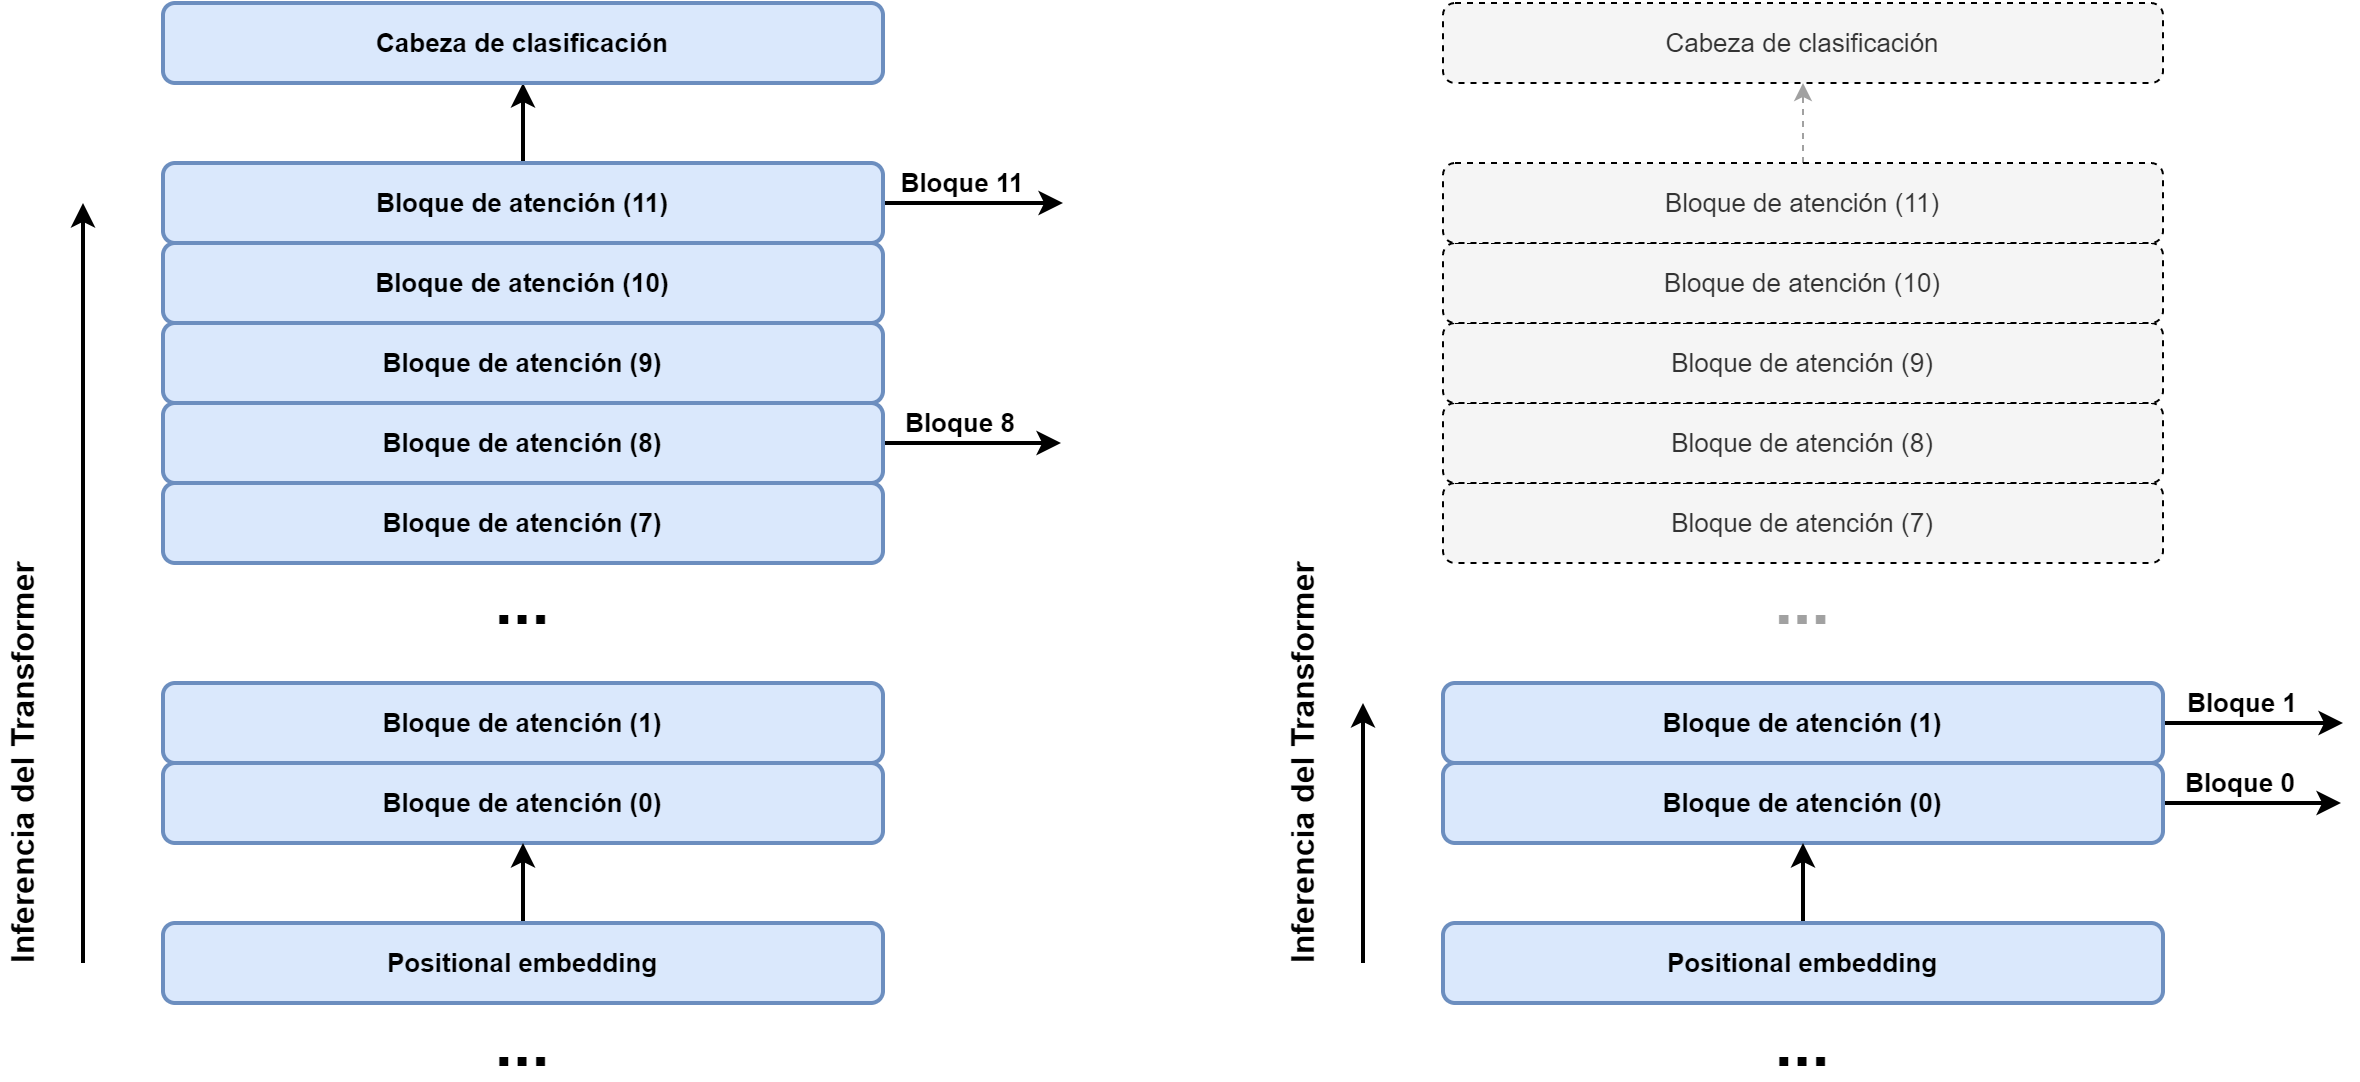
\includegraphics[width=\textwidth]{imagenes/DPT-cambio-bloques-transformer.png}
\caption{Cambio en el número de bloques de atención.}
\label{fig:attention_block_num}
\end{figure}



\begin{figure}[H]
\centering
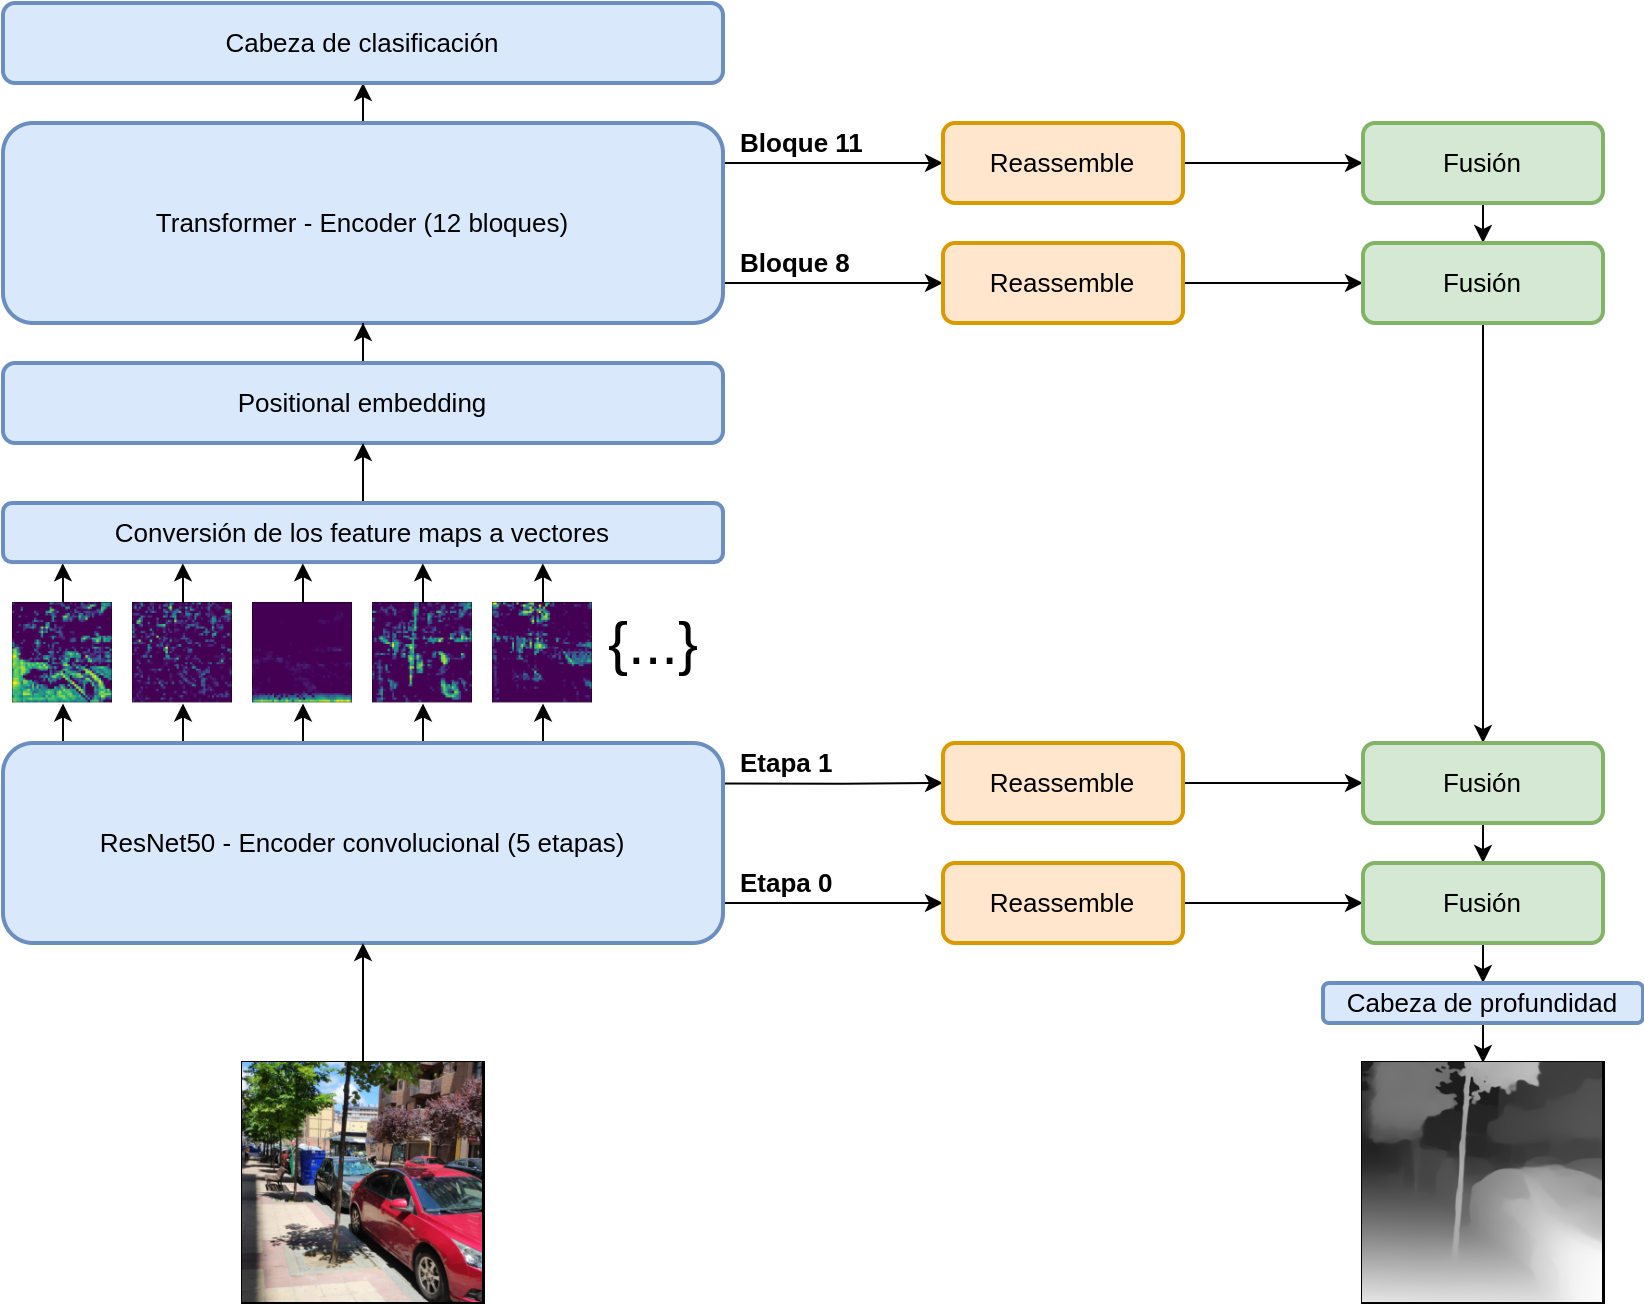
\includegraphics[width=\textwidth]{imagenes/DPT-general.png}
\caption{Arquitectura general DPT.}
\label{fig:dpt-general}
\end{figure}

\begin{figure}[H]
\centering
\includegraphics[width=\textwidth]{imagenes/DPT-modificado-general.png}
\caption{Arquitectura general DPT tras las modificaciones.}
\label{fig:dpt-mod-general}
\end{figure}

\subsection{Cambio del backbone convolucional}
El último cambio estudiado en este proyecto es el del backbone convolucional del Hybrid ViT. En el modulo propuesto en la publicación original, se elige como backbone una ResNet50v2, de la que se extraen las activaciones en los bloques 0 y 1, que tienen un tamaño TODO de 256 y 512, quedando así TODO de tamaños [256, 512, 768, 768]. Por otro lado, la salida de la última capa de la ResNet50v2, es decir, la entrada de los bloques de atención, tiene forma [n, c, h, w], donde n es el número de imágenes en el batch (batch size), c el número de canales (en este caso mapas de características), que son 1024 por como está diseñada la arquitectura, y por último, h y w, que son la altura y anchura de los mapas de características y son iguales a las dimensiones de la imagen de entrada divididas 4 veces entre 2. Después de la ResNet, hay una capa de proyección que no es más que una capa convolucional con kernels de tamaño 1x1 y stride 1x1, con 1024 canales de entrada y 768 canales de salida. Este tipo de capas, realmente son 786 kernels de 1x1x1024, por lo que al convolucionar cada uno de ellos la entrada, se obtienen 768 mapas de características del mismo tamaño que los de la entrada. Los 768 mapas de características resultantes, se aplanan en tensores de forma [n, 768, h/8 * w/8] y se transponen de forma que la entrada sea de tipo [n, t, 768], donde 768 es el tamaño de los tokens de los bloques de atención y t el número de tokens extraidos de la imagen. De esta forma, a mayor tamaño de imagen mayor será el número de tokens, pero la dimensión de estos permanece constante.

\todo[inline]{Hablar de las convoluciones con kernels 1x1 arriba en vez de aquí?}

A modo de ejemplo, supongamos una entrada de una sola imagen de tamaño 384x384: la salida de la ResNet50v2 tendrá la forma [1, 1024, 24, 24]. Esta salida atraviesa la capa de proyección y pasa a tener forma [1, 768, 24, 24]. Estos mapas de características se aplanan en un tensor [1, 768, 576] que se traspone para obtener la forma [1, 576, 768], que equivale a 576 tokens de dimensión 768. Una vez llegados a este punto, el tensor está listo para pasar a los bloques de atención del transformer.

Por otro lado, la arquitectura EfficientNet-B0, alternativa usada en las pruebas de este trabajo, proporciona una salida (antes de la capa de global pooling) de forma [n, c, h, w] donde n vuelve a ser el número de imágenes procesadas en paralelo, el número de mapas de características es en este caso 1280, y la altura y anchura se corresponden con las de las imágenes de entrada divididas 5 veces entre 2. Es decir: [n, 1280, h/16, w/16]. Para poder sustituir el backbone convolucional del Hybrid ViT sin tener que cambiar el tamaño de todas las capas de atención (para poder aprovechar los pesos preentrenados), se sustituye la capa de proyección mencionada en el párrafo superior, que recordemos era una capa convolucional con kernels de tamaño 1x1 por una capa de convolución transpuesta. Esta capa de convolución transpuesta, cumple dos funciones fundamentales: la primera, transforma los 1280 mapas de características en 768; y la segunda, al tener un kernel de tamaño 2x2 y un stride también de 2x2, consigue que las dimensiones de estos mapas de características se multiplen exactamente por 2 en ambas dimensiones, convirtiendo la entrada [n, 1280, h/16, w/16] en [n, 1280, h/8, w/8], que es lo que espera la etapa que aplana los mapas de características y transpone el tensor para obtener de nuevo la entrada preparada para los bloques de atención de forma [n, t, 768] donde t vuelve a ser el número de tokens que pasan al transformer, cada uno de dimensión 768.

\todo[inline]{Explicar bien y añadir en el parrafo de efficientnet el tamaño que tienen los hooks de la red convolucional}
\todo[inline]{Meter alguna imagen para explicar todo este apartado}
\todo[inline]{Decir lo de que se ha modificado la carga de pesos del modelo}
\todo[inline]{Decir (y luego repetir) que efficientnet no está preentrenada en mix y que esto evidentemente afectará a los resultados}


% En los resultados hablar de la distribución de los pesos antes y después de convertir el modelo si es pertinente, hacer una especie de estudio de ablación si se puede entrenar modelos, etc. Puede estar interesante quitar cabezas de atención, quitar bloques de atención, ver como afecta al tamaño dle modelo, su rendimiento (velocidad y métricas)...

\clearpage